\myChapter{Iniezione di attacchi in CARLA}
Il lavoro svolto è stato il seguente:  l'individuazione di attacchi dell'ART interessanti da analizzare e implementare, iniettandoli all'interno di un modello preesistente di guida
autonoma che gira su CARLA. In questo capitolo vengono descritti:\begin{itemize}
    \item il modello scelto
    \item gli attacchi scelti
    \item iniezione e risultati
\end{itemize}
\section{Il modello scelto}
Per semplicità implementativa è stato scelto un modello preaddestrato. La scelta è ricaduta su Learning By Cheating (LBC) \cite{lbc}. LBC utilizza l'imitation learning come
approccio e divide la fase di addestramento in due parti: \begin{itemize}
    \item nella prima viene addestrato un agente privilegiato sulla base di traiettorie di esperti. Questo agente ha accesso a tutte le informazioni 
    dell'ambiente circostante (layout ambientale, posizione di ogni altro partecipante). Agisce sull'ambiente con una vista dall'alto (birdview).
    \item nella seconda fase l'agente privilegiato fa da supervisore per l'addestramento di un agente sensorimotore. Questo ha accesso soltanto alle informazioni dei
    propri sensori (una camera RGB frontale). Viene addestrato per imitare l'agente privilegiato.
\end{itemize}
L'apprendimento è stato suddiviso in due fasi per separare due compiti: imparare ad \emph{agire}, compito dell'agente privilegiato e imparare a \emph{vedere}, compito dell'agente sensorimotore.
Tale suddivisione porta i seguenti vantaggi:\begin{itemize}
    \item poichè l'agente privilegiato utilizza una rappresentazione compatta dell'ambiente, apprende più velocemente e generalizza meglio;
    \item la supervisione fornita dall'agente privilegiato è di gran lunga più forte rispetto alle traiettorie originali, perchè può essere interrogato 
    su qualsiasi stato dell'ambiente;
    \item l'agente privilegiato è di tipo white box e il suo stato interno può essere analizzato in qualsiasi istante.
\end{itemize}
Nella Figura \ref{fig:arch} è mostrata l'architettura dei due agenti. Concentrandosi sull'agente sensorimotore, l'input viene passato a una rete convoluzionale che produce una serie di 
traiettorie nella camera frontale. Le traiettorie  sono selezionate sulla base del comando scelto e vengono passate al controllore di basso livello che produce un valore di sterzata, accelerazione o freno.
\begin{figure}[h!]
    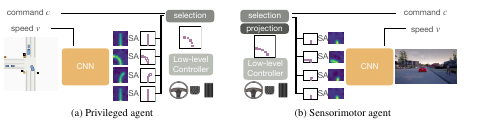
\includegraphics[width=\linewidth]{agenti.png}
    \caption{Architettura dei due agenti \cite{lbc}.}
    \label{fig:arch}
\end{figure}


\section{Gli attacchi scelti}
Tra gli attacchi presenti nell'ART sono stati analizzati solamente gli evasion attacks per i seguenti motivi:\begin{itemize}
    \item utilizzando un modello preaddestrato ha poco senso andare a implementare i poisoning attacks, in quanto essi agiscono durante la fase di training
    \item gli extraction attacks sono stati esclusi in quanto LearningByCheating è open-source mentre questo tipo di attacchi sono rilevanti quando si ha a che fare
    con algoritmi proprietari
\end{itemize}
Tra gli attacchi analizzati ne abbiamo individuati tre di particolare interesse:\begin{itemize}
    \item Adversarial Patch
    \item Spatial Transformation
    \item HopSkipJump
\end{itemize}
\subsection{Adversarial Patch} 

\subsection{Spatial Transformation}

\subsection{HopSkipJump}

\section{Iniezione degli attacchi}
LearningByCheating fornisce un modulo (run\_benchmark) grazie al quale valutare un agente sensorimotore (benchmark\_agent) su una serie di percorsi prestabiliti.
In questi percorsi l'agente deve arrivare a un punto della mappa preciso entro un tempo limite. Per ciascun percorso viene tenuto traccia dei semafori rossi ignorati, delle invasioni di corsia e delle collisioni. Inoltre viene registrato un video che mostra il veicolo mentre percorre il tragitto.
Nel video vengono mostrati anche gli waypoints generati dalla rete neurale in ogni momento. Nel Listing \ref{run} viene definito il loop principale di un percorso.
Ad ogni intervallo di simulazione ( $env.tick()$ aspetta l'esecuzione di un'azione),  l'agente riceve le osservazioni dai sensori ($env.get\_observations()$), le passa alla 
rete neurale che decide l'azione ($agent.run\_step(observations)$) e applica l'azione restituita attraverso i controllori ($env.apply\_control(control)$). Il percorso termina 
se il veicolo arriva a destinazione, scade il tempo, oppure avviene una collisione. L'ultima condizione non era presente nel codice originale ma è stata aggiunta per risparmiare tempo sulla singola run nel caso in cui avvenga un incidente. Per essere efficaci gli attacchi devono modificare gli input 
\textbf{prima} che arrivino alla rete, quindi la riga $agent.run\_step(observations)$ è stata individuata come il punto giusto nel quale iniettare gli attacchi prescelti.

Il metodo $run\_step$ è definito nella classe ImageAgent del  modulo $image$ ( Listing \ref{img}).

La perturbazione dell'immagine avviene in:
\begin{lstlisting}[language=Python]
    _rgb= self.attack.generate(x=_rgb.cpu())
    _rgb = torch.FloatTensor(_rgb)
\end{lstlisting}
Il metodo $generate$ attua la modifica vera e propria dell'immagine. Il campo $self.attack$ rappresenta l'attacco iniettato. L'iniezione avviene nelle due righe aggiunte al costruttore:
\begin{lstlisting}[language=Python]
    self.adv = load_model('/home/piazzesi/Desktop/carla_lbc/ckpts/image')
    self.attack = load_attack(self.adv, 'hopskipjump')
\end{lstlisting}
Le funzioni $load\_model$ e $load\_attack$ sono state implementate nel modulo $attack$ (Listing \ref{att}). Si nota come la definizione  degli attacchi corrisponde semplicemente a una chiamata
di un costruttore. L'implementazione vera e propria  è fornita direttamente dai moduli dell'ART.

Le ultime modifiche sono state attuate nel metodo $forward$ della classe $ImagePolicyModelSS$ (Listing \ref{for}). Questa classe è l'implementazione della rete neurale e in $forward$ avviene il processo decisionale.
$forward$ viene anche usato nel metodo $generate$ per realizzare la perturbazione. Il problema è che $generate$ prende come unico parametro l'immagine RGB mentre $forward$ usa anche velocità e comando.
La soluzione scelta è stata la seguente: la velocità e il comando non vengono passati a $forward$ attraverso i  parametri di input, ma vengono recuperati  dalle variabili globali $\_speed$ e $\_command$ definite in $run\_step$. Usare variabili globali
non è sicuramente una pratica di buona programmazione, ma ha permesso l'esecuzione degli attacchi senza problemi. Infine, sempre per garantire la compatibilità tra ART  e modello è stata aggiunta la riga:
\begin{lstlisting}[language=Python]
    location_pred = torch.reshape(location_pred,(1,10))
\end{lstlisting}
La modifica è necessaria perchè il tensore location\_pred è della forma [2, 5] (bidimensionale con 5 elementi per dimensione). L'ART non supporta output multidimensionali, dunque il tensore viene convertito nella forma [1, 10].

L'intero codice modificato è disponibile a \href{https://github.com/piazzesiNiccolo/myLbc}{\emph{questo link.}}
\lstinputlisting[language=Python,caption=loop base di una run,label=run]{code/run_benchmark.py}
\lstinputlisting[language=Python, caption=ImageAgent,label=img]{code/image.py}
\lstinputlisting[language=Python,caption=attack.py,label=att]{code/attack.py}
\lstinputlisting[language=Python,caption=ImagePolicyModelSS,label=for]{code/image_model.py}

\section{Risultati}
Per confrontare gli attacchi è stato eseguito $run\_benchmark$ sulla suite $regular$.
Questa suite è composta da 4 gruppi di percorsi basati sulle mappe NoCrashTown01 e NoCrashTown02. Ogni gruppo fornisce un percorso ripetuto tre volte con diverse condizioni meteorologiche.
Un percorso viene considerato non completato se avviene una collisione oppure se il veicolo non arriva al goal entro il limite di tempo (timeout).

Il percorso in NoCrashTown01 prevede una singola curva a destra, mentre in NoCrashTown02 sono presenti svolte e incroci multipli.
I 4 gruppi hanno le seguenti caratteristiche:\begin{itemize}
    \item NoCrashTown01-v3\begin{itemize}
        \item condizioni metereologiche: ClearNoon (mezzogiorno, nuvoloso con asfalto asciutto), WetNoon (mezzogiorno, nuvoloso con asfalto bagnato) e HardRain (mezzogiorno, pioggia intensa con asfalto bagnato)
        \item numero di veicoli:20
        \item numero di pedoni:50
    \end{itemize}
    \item NoCrashTown02-v3 \begin{itemize}
        \item condizioni metereologiche: ClearNoon, WetNoon e HardRain 
        \item numero di veicoli:15
        \item numero di pedoni:50
    \end{itemize}
    \item NoCrashTown01-v4 \begin{itemize}
        \item condizioni metereologiche: WetSunset (tramonto, sereno con asfalto bagnato) e SoftRainSunset (tramonto, pioggia debole  con asfalto bagnato). WetSunset è usato in due percorsi.
        \item numero di veicoli:20
        \item numero di pedoni:50
    \end{itemize}
    \item NoCrashTown02-v4 \begin{itemize}
        \item condizioni metereologiche: WetSunset  e SoftRainSunset.
        \item numero di veicoli:15
        \item numero di pedoni:50
    \end{itemize}
\end{itemize}

La valutazione degli attacchi si è svolta in due fasi:\begin{itemize}
    \item nella prima, i percorsi sono stati seguiti da un agente senza nessun attacco iniettato (golden run);
    \item nella seconda fase, si eseguono le stesse run della prima, ma ogni volta con un diverso attacco iniettato.
\end{itemize}
I risultati prodotti dall'iniezione di ciascun attacco sono stati confrontati con quelli prodotti dalla golden run, in modo da valutarne l'efficacia.
Il confronto è stato fatto con l'analisi dei video prodotti, valutando i percorsi portati a termine,  la stabilità della guida, i semafori rossi ignorati e le cause dei percorsi
non completati(collisioni e timeout).
\subsection{Golden Run}
\begin{table}[h]
    \begin{tabular}{|c|c|c|}
        \hline
        Mappa                   & Run completate & Percentuale di completamento\\
        \hline
        NoCrashTown01-v3        & 3/3            & 100\% \\
        NoCrashTown01-v4        & 3/3            & 100\% \\
        NoCrashTown02-v3        & 3/3            & 100\% \\
        NoCrashTown02-v4        & 3/3            & 100\%  \\
        \hline
        \textbf{TOTALE}                  & 12/12          & 100\% \\
        \hline
    \end{tabular}
    \caption{risultati golden run}
Nella golden run tutti i percorsi vengono completati con successo. La traiettoria del veicolo è stabile, nessun semaforo è stato ignorato e non si sono registrate collisioni.
\end{table}
\begin{figure}[h!]
    \centering
    \parbox{6cm}{
    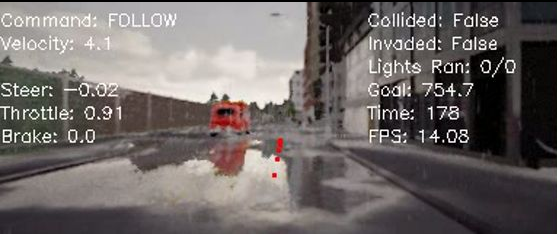
\includegraphics[width=6cm]{GOLD1.png}
    \label{fig:gold1}}
    \qquad
    \begin{minipage}{6cm}
    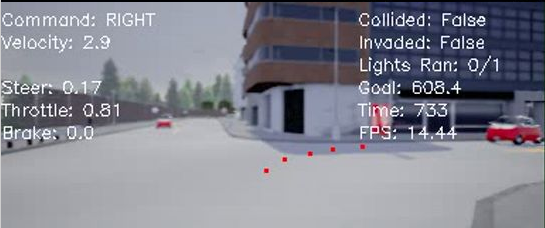
\includegraphics[width=6cm]{GOLD2.png}
    \label{fig:gold2}
    \end{minipage}
    \caption{golden run}
    \label{fig:goldrun}
    \end{figure}
\newpage
\subsection{Iniezione di HopSkipJump (HSJ)}
\begin{table}[h]
    \begin{tabular}{|c|c|c|}
        \hline
        Mappa                   & Run completate & Percentuale di completamento\\
        \hline
        NoCrashTown01-v3        & 3/3            & 100\% \\
        NoCrashTown01-v4        & 2/3            & 66\% \\
        NoCrashTown02-v3        & 1/3            & 33\% \\
        NoCrashTown02-v4        & 0/3            & 0\%  \\
        \hline
        \textbf{TOTALE}                  & 6/12           & 50\% \\
        \hline
    \end{tabular}
    \caption{risultati run HopSkipJump}
    \label{tab:hsj}
\end{table}
La macchina continua a seguire il percorso prestabilito in modo molto più instabile. L'instabilità è particolarmente evidente negli waypoints generati, che cambiano continuamente posizione anche nei rettilinei. A causa dei problemi elencati
si nota un aumento dei semafori ignorati(9) e delle uscite fuori strada. I fallimenti(6) sono stati tutti causati da collisioni.
\begin{figure}[h]
    \centering
    \parbox{6cm}{
    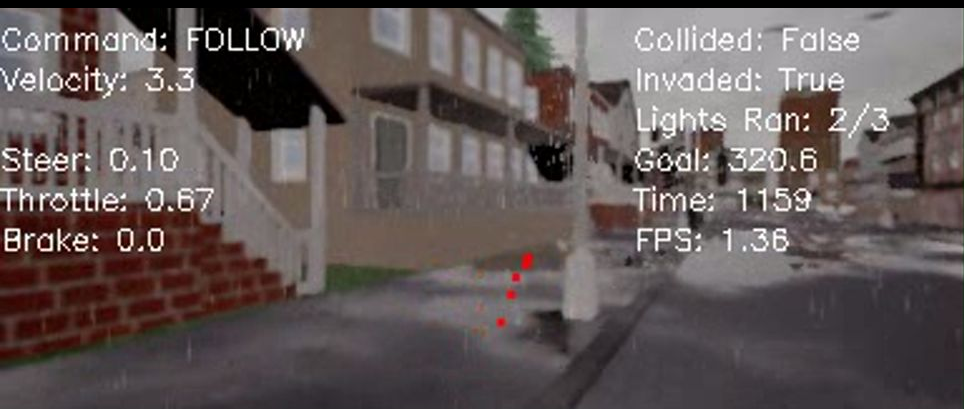
\includegraphics[width=6cm]{hoprun.png}
    \label{fig:hop1}}
    \qquad
    \begin{minipage}{6cm}
    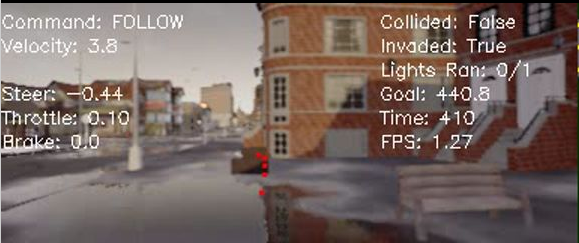
\includegraphics[width=6cm]{HOP2.png}
    \label{fig:hop2}
    \end{minipage}
    \label{fig:hoprun}
    \caption{collisioni causate da HopSKipJump}
    \label{fig:hop}
    \end{figure}
\subsection{Iniezione di Spatial Transformation}
\begin{table}[h]
    \begin{tabular}{|c|c|c|}
        \hline
        Mappa                   & Run completate & Percentuale di completamento\\
        \hline
        NoCrashTown01-v3        & 2/3            & 66\% \\
        NoCrashTown01-v4        & 3/3            & 100\% \\
        NoCrashTown02-v3        & 1/3            & 33\% \\
        NoCrashTown02-v4        & 1/3            & 33\%  \\
        \hline
        \textbf{TOTALE}                  & 7/12           & 0\% \\
        \hline
    \end{tabular}
    \caption{risultati run Spatial Transformation (STA)}
    \label{tab:sta}
\end{table}
Nelle run completate la macchina si comporta normalmente. Non si notano variazioni rilevanti nella traiettoria e nessun semaforo viene ignorato. Delle 5 run
non completate, quattro sono terminate per collisione avvenuta e una per timeout. In queste run si nota una tendenza del veicolo ad andare largo alle curve, fino ad invadere la corsia opposta e causare un incidente.
In una run la macchina esce subito di strada andando a sbattere contro un edificio nelle vicinanze.
\begin{figure}[h]
    \centering
    \parbox{6cm}{
    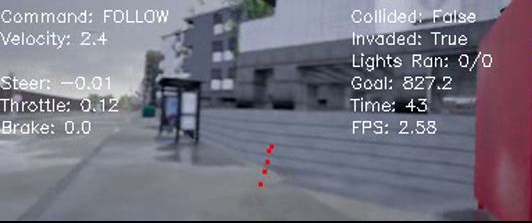
\includegraphics[width=6cm]{STA1.png}
    \label{fig:sta1}}
    \qquad
    \begin{minipage}{6cm}
    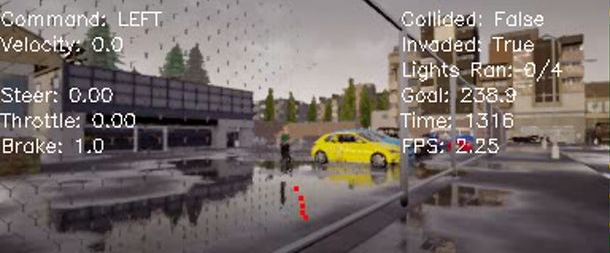
\includegraphics[width=6cm]{STA2.png}
    \label{fig:sta2}
    \end{minipage}
    \caption{collisioni causate da Spatial Transformation}
    \label{fig:starun}
    \end{figure}
\subsection{Iniezione di Basic Iterative Method(BIM)}
\begin{table}[h]
    \begin{tabular}{|c|c|c|}
        \hline
        Mappa                   & Run completate & Percentuale di completamento\\
        \hline
        NoCrashTown01-v3        & 0/3            & 0\% \\
        NoCrashTown01-v4        & 0/3            & 0\% \\
        NoCrashTown02-v3        & 0/3            & 0\% \\
        NoCrashTown02-v4        & 0/3            & 0\%  \\
        \hline
        \textbf{TOTALE}                  & 0/12           & 0\% \\
        \hline
    \end{tabular}
    \caption{risultati run Basic Iterative Method}
    \label{tab:bim}
\end{table}
La guida autonoma risulta compromessa. In nessuno dei percorsi la macchina segue il tragitto, ma invece sterza subito verso destra fino ad uscire di strada
e urtare oggetti della mappa.
\begin{figure}[h]
    \centering
    \parbox{5cm}{
    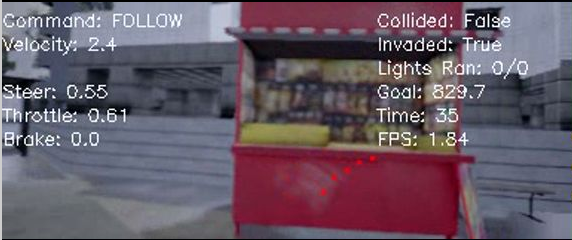
\includegraphics[width=5cm]{BIM1.png}
    \label{fig:bim1}}
    \qquad
    \begin{minipage}{5cm}
    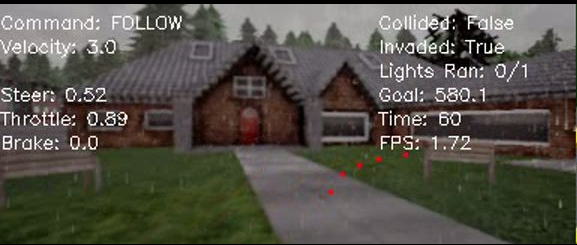
\includegraphics[width=5cm]{BIM2.png}
    \label{fig:bim2}
    \end{minipage}
    \caption{collisioni causate da Basic Iterative Method}
    \label{fig:bimrun}
    \end{figure}
\newpage
\subsection{Iniezione di NewtonFool (NF)}
\begin{table}[h!]
    \begin{tabular}{|c|c|c|}
        \hline
        Mappa                   & Run completate & Percentuale di completamento\\
        \hline
        NoCrashTown01-v3        & 1/3            & 33\% \\
        NoCrashTown01-v4        & 2/3            & 66\% \\
        NoCrashTown02-v3        & 0/3            & 0\% \\
        NoCrashTown02-v4        & 0/3            & 0\%  \\
        \hline
        \textbf{TOTALE}                  & 3/12           & 25\% \\
        \hline
    \end{tabular}
    \caption{risultati run NewtonFool}
    \label{tab:nf}
\end{table}
Il veicolo diventa inaffidabile. Si ha bassa stabilità nella guida e nella traiettoria generata. Le run non completate(9) sono state tutte causate da collisioni dopo che la macchina
aveva invaso la corsia opposta o era uscita di strada. \begin{figure}[h]
    \centering
    \parbox{6cm}{
    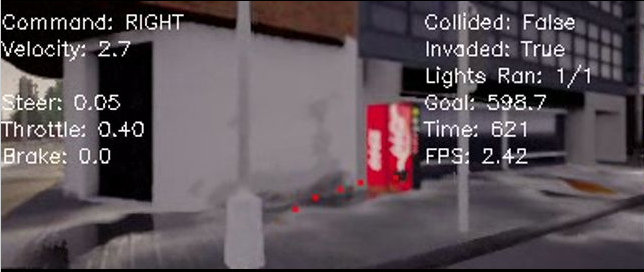
\includegraphics[width=6cm]{FOOL1.png}
    \label{fig:fool1}}
    \qquad
    \begin{minipage}{6cm}
    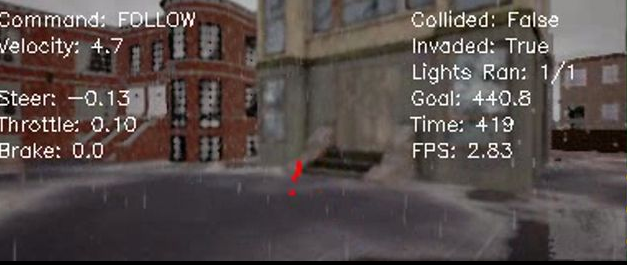
\includegraphics[width=6cm]{FOOL2.png}
    \label{fig:fool2}
    \end{minipage}
    \caption{collisioni causate da NewtonFool}
    \label{fig:foolrun}
    \end{figure}
\newpage
\subsection{Sintesi risultati}
I risultati raccolti (riassunti nella Tabella \ref{tab:ria}) confermano la vulnerabilità del modello considerato agli adversarial attacks. In tutti i casi l'affidabilità del veicolo si è ridotta.
L'attacco che ha causato problemi più gravi è sicuramente Basic Iterative Method. Mentre nelle altre run la traiettoria prestabilita continua ad essere quantomeno seguita, in questo
caso la macchina cambia completamente comportamento, diventando inutilizzabile.
\begin{table}[h]
    \begin{tabular}{|p{1.5cm}|p{2.5cm}|p{2cm}|p{1.5cm}|c|c|}
        \hline
        Attacco        &   Run completate     &   stabilità     &  semafori ignorati        & collisioni & timeout\\
        \hline
        Nessuno        &  12/12               &   ottima        &  0                       & 0          & 0 \\
        HSJ            &  6/12                &   bassa         &  9                        & 6          & 0 \\
        STA            &  7/12                &   discreta      &  0                        & 4          & 1 \\
        BIM            &  0/12                &   nulla         &  N/D                      & 12         & 0\\
        NF             &  3/12                &   bassa         &   13                      & 9          & 0 \\
        \hline
    \end{tabular}
    \caption{riassunto dei risultati}
    \label{tab:ria}
\end{table}